Pour la réalisation du projet informatique, notre équipe a choisi d'adopter une méthode agile. Cette méthode nous a permis de progresser efficacement en planifiant les tâches de manière itérative. 
Chaque semaine, généralement lors de la séance de TD, nous avons tenu une réunion d'avancement. Cette réunion était divisée en deux parties, on discutait d'abord des tâches accomplies lors de la semaine passée puis des prochaines taches à réaliser. 
Notre chef de projet, Donovann, prenait ensuite en charge la planification et l'affectation des tâches à réaliser dans la semaine, en s'assurant que celles-ci étaient claires et bien définies.

\vspace{3mm}
\begin{figure}[H]
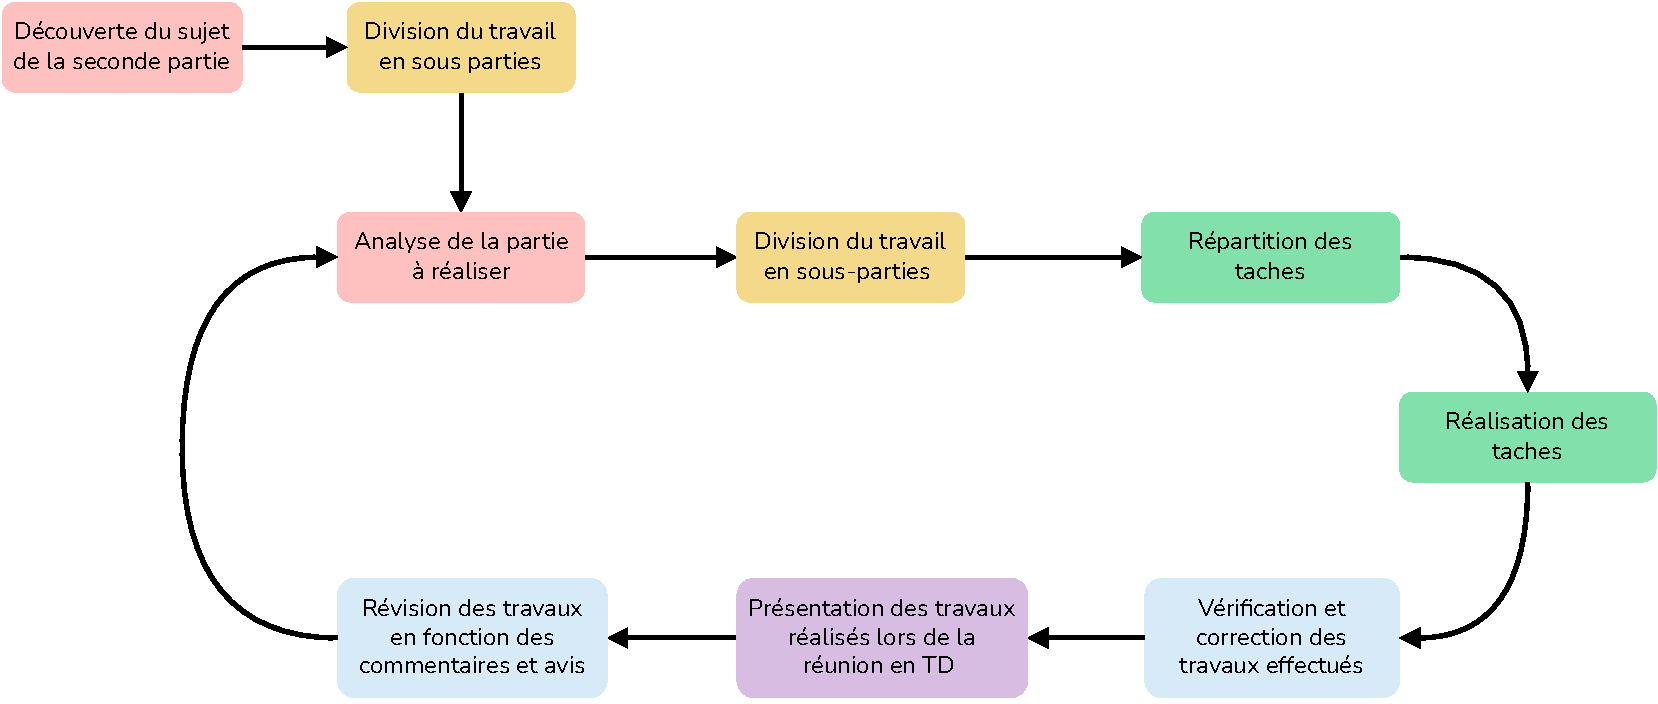
\includegraphics[width=\textwidth]{Organisation.pdf}
\caption{Diagramme des étapes de réalisation du projet}
\end{figure}
\vspace{2mm}

Afin de faciliter la collaboration au sein de l'équipe ainsi que le suivi du projet, nous avons utilisé plusieurs outils. Tout d'abord, nous avons choisi Github comme plateforme de gestion de versions pour stocker le code et suivre les modifications apportées par chaque membre de l'équipe au fil du temps. Cela nous a permis de collaborer plus efficacement et de garder une trace de l'évolution du projet.\\

Nous avons également utilisé un serveur Discord pour les communications inter-équipe, ce qui nous a permis d'organiser les discutions en différentes catégories (discussions techniques, questions, gestion du projet,...).\\

Dans l'ensemble, l'utilisation de ces outils nous a permis de travailler de manière plus efficace et d'améliorer la collaboration tout au long du projet. Les informations relatives à nos outils sont accessibles via les liens \href{https://github.com/}{Github}, \href{https://www.jetbrains.com/fr-fr/pycharm/}{PyCharm}, \href{https://www.jetbrains.com/fr-fr/webstorm/}{WebStorm} et \href{https://discord.com/}{Discord}.


\begin{landscape}
\begin{figure}[htbp]
\vspace{4mm}

  \centering
  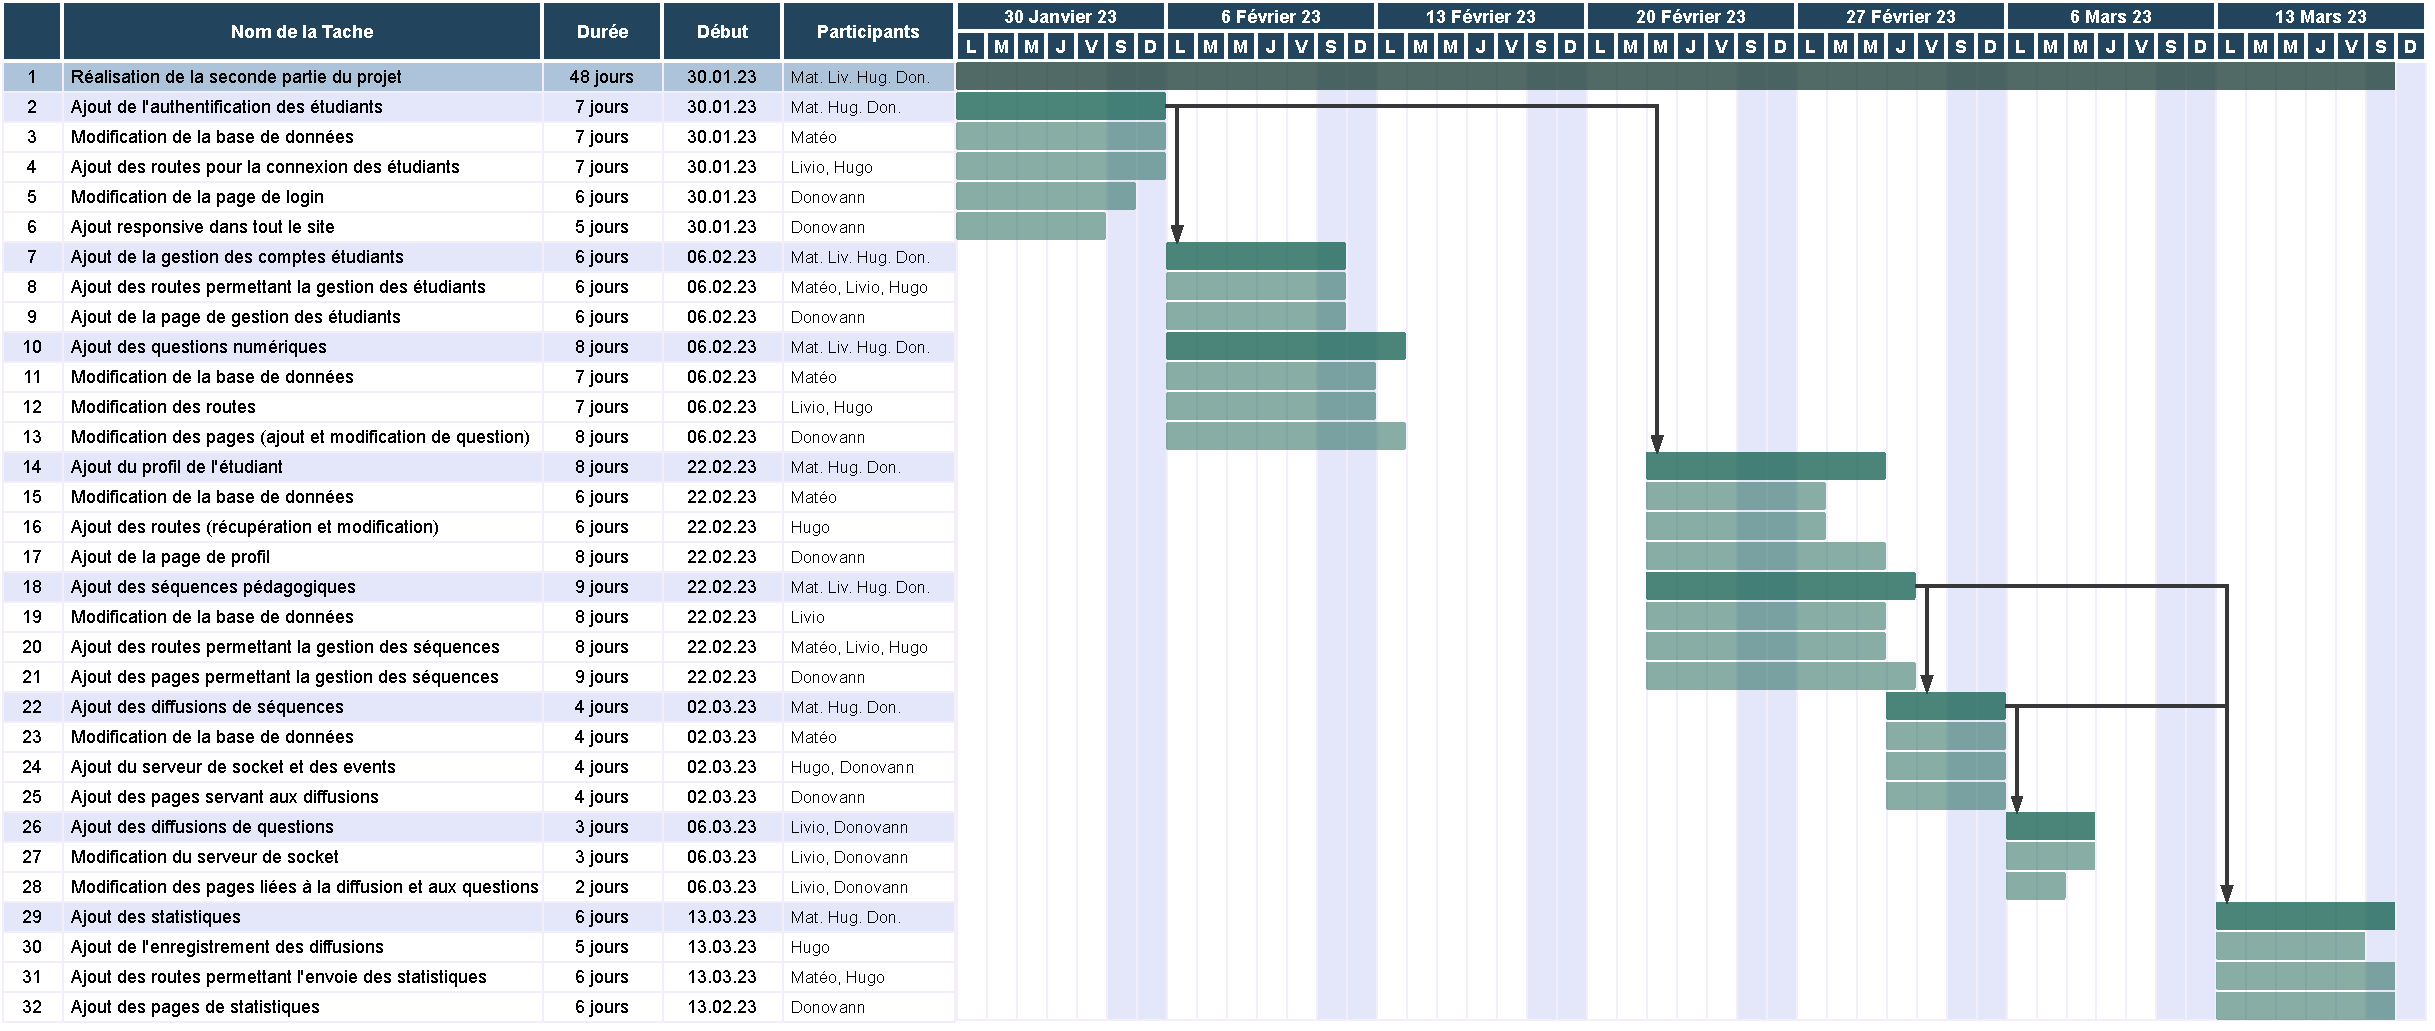
\includegraphics[width=\linewidth]{Gantt.pdf}
  \caption{Diagramme de Gantt du projet}
\label{fig:pdf-horizontal}
\end{figure}

Ce diagramme de Gantt est une représentation visuelle des étapes du projet. 
Les étapes du projet sont représentées par des barres horizontales. 
Chaque étape principale (vert foncé) peut comporter une ou plusieurs étapes secondaires (vert). 
Les flèches, quant à elles, indiquent les dépendances entre les étapes.\\\\

Il est important de noter que la réalisation de la vidéo présentant les fonctionnalités du site, ainsi que la rédaction du rapport, n'ont pas été prises en compte dans le diagramme de Gantt car elles ne faisaient pas partie intégrante du projet. Cependant, le projet a été planifié pour laisser suffisamment de temps pour la production de la vidéo ainsi que la rédaction du rapport.
\end{landscape}
